% !TeX root = RJwrapper.tex
\title{remap: Regionalized Models with Spatially Smooth Predictions}
\author{by Jadon Wagstaff and Brennan Bean}

\maketitle

% 150 words
\abstract{
Traditional spatial modeling approaches assume that data are second-order stationary, which is rarely true over large geographical areas. A simple way to model nonstationary data is to partition the space and build models for each region in the partition. This has the side effect of creating discontinuities in the prediction surface at region borders. The regional border smoothing approach ensures continuous predictions by using a weighted average of predictions from regional models. The R package \pkg{remap} is an implementation of regional border smoothing that builds a collection of spatial models. Special consideration is given to distance calculations that make \pkg{remap} package scalable to large problems. Using the \pkg{remap} package, as opposed to global spatial models, results in improved prediction accuracy on test data. These accuracy improvements, coupled with their computational feasibility, illustrate the efficacy of the \pkg{remap} approach to modeling nonstationary data.
}

\section{Introduction}

When observations exhibit spatial autocorrelation, geographic location can be leveraged to improve predictions of the response variable by considering responses in nearby observations. Typical spatial statistical models assume that the covariance between two observations can be modeled as a function of location difference, i.e., the relationship needs to be second-order stationary. For sufficiently large distances, the stationarity assumption often fails. Even when external drift or secondary variables are used, continental scale models may still not be second-order stationary.

The simplest way to use traditional spatial modeling with nonstationary data is to partition the global region into smaller sub-regions that are locally stationary and create separate models for each region. The na\"ive implementation of this approach leads to noncontinuous predictions at the borders of each region. Previous attempts to smooth out discontinuities at region boundaries often involved taking weighted averages of local regional model output where the weights of each local model prediction or covariance structure are a function of the distance between a new observation and the centers of each region \citep{fuentes_high_2001, fuentes_new_2001, gosoniu_bayesian_2006, gosoniu_mapping_2009, konomi_adaptive_2014}. While the center based approach may be appropriate for symmetrical regions, it is likely not appropriate for oddly shaped or disjoint regions not well represented by their centers. In some cases, a region may not even contain its center. The center-based approach also fails to respect major geographic features that can cause sharp changes in response variables over very short distances. 

The regional border smoothing approach described in this article is a novel method that uses a weighted average of predictions from local models, but gives weight to regional models based on the nearest distance to the \emph{border} of each region rather than distance to the center of each region. With this method, regions may be chosen that more naturally reflect local climate and topography with smoothing only occurring near the borders of each region. Figure \ref{fig:example} is an example of the regional border smoothing approach applied to three regions with different spatial models.

\begin{figure}[htbp]
    \centering
    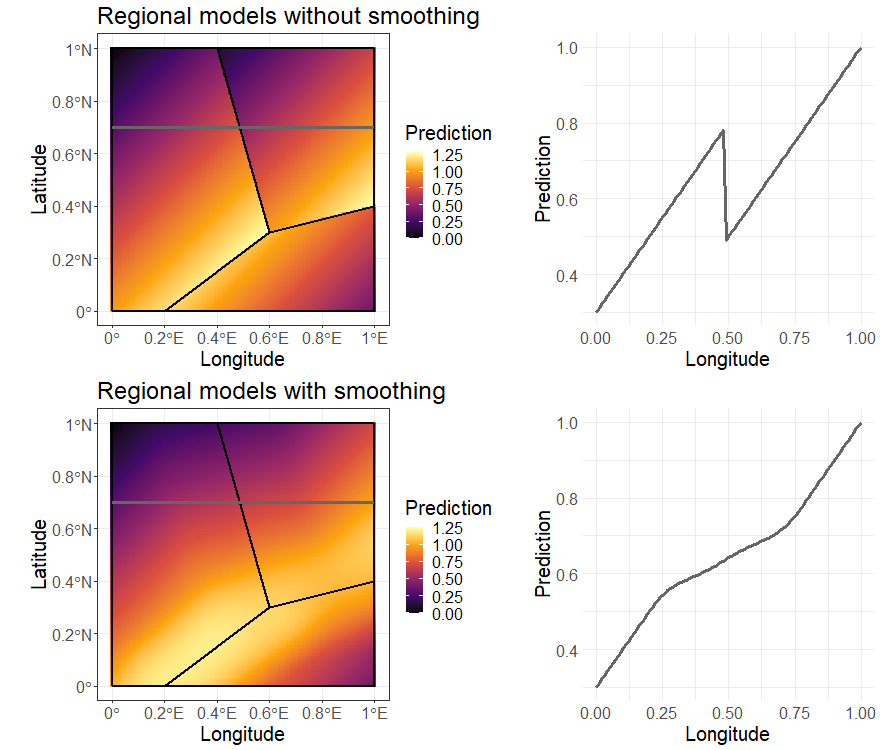
\includegraphics[width = \textwidth]{figures/example.png}
    \caption{With (bottom) and without (top) application of regional border smoothing where predictions are a linear combination of longitude and latitude. The gray line shows predicted values at 0.7\textdegree N. Left region predicts $lon - lat + 1$, bottom region predicts $lat - lon + 1.4$, and right region predicts $lon - lat + 0.7$. Smoothing zone is 30 km ($\approx 0.27$\textdegree).}
    \label{fig:example}
\end{figure}

The R package \CRANpkg{remap} is a General Public License implementation of this regional border smoothing method that scales well to large problems \citep{remap}. Using \pkg{remap}, regional border smoothing is applied to two different modeling problems. The first problem is a national set of 50-year ground snow loads and the second problem is modeling April 1st snow water content for Utah. Mapped values from both projects show improvement in model accuracy using the regional border smoothing approach over global models for a variety of spatial modeling approaches.

The body of this article will proceed with a description of the regional border smoothing approach. This will be followed by an illustration of the available functions and tools in \pkg{remap} as well as two demonstrations of the software on a state and national-level data set. These examples show the utility of \pkg{remap} in producing smooth estimates when applied to spatial modeling problems over large geographical areas with irregularly shaped partitions.

\subsection{Background}

There are many proposed methods to model nonstationary data using locally stationary models. \citet{haas_lognormal_1990, haas_kriging_1990} describes a moving window approach where only data within a pre-specified bounding box are used to fit a local dependence structure and then make predictions. This process is computationally intensive and may not result in continuous predictions. 

\citet{fuentes_high_2001} and \citet{fuentes_new_2001} propose a method for nonstationary problems where a global covariance structure that changes continuously as a function of location is used in a Gaussian process model. The data are first partitioned into locally stationary regions and a global covariance structure is calculated by taking a weighted average of regional covariance structures. Weights are based on the distance from the prediction location to a point in each region, usually the center. Regions are either given \emph{a priori} or by using subgrids chosen using the Bayesian information criterion.

Applications of local partition modeling approaches include \citet{kim_analyzing_2005}, who describe a method to deal with sudden changes in spatial covariance structure that occur between layers of rock strata. The spatial domain is partitioned into independent regions using Voronoi Tessellations \citep{green1978}, with each region fit using an independent Gaussian model. The resulting global model has sharp changes at the borders of each region, which was desirable given the context of the problem. \citet{konomi_adaptive_2014} illustrate a decision tree based method for partitioning the spatial domain when modeling global Ozone levels. \citet{heaton_nonstationary_2017} use a hierarchical clustering method to partition the spatial domain for temperature data in Houston, TX. The hierarchical clustering method has the benefit of creating a partition that more naturally follows changes in the covariance structure rather than partitioning the space into symmetrical blocks or spheres.

\citet{gosoniu_bayesian_2006, gosoniu_mapping_2009} provide an additional application of local partitioning models mapping malaria risk using \emph{a priori} partitions of West Africa. The 2006 study uses three large rectangular regions and the 2009 study uses agro-ecological regions to partition the spatial domain. In these studies, spatial random effects are modeled as a weighted sum of regional stationary effects based on the distance to region centroids. The authors note problems with sudden changes at region borders as a result of using region centroids for the weighted sum of effects.

Most of the methods discussed so far create a global covariance structure from local covariance structures of Gaussian process models \citep{fuentes_high_2001, fuentes_new_2001, kim_analyzing_2005, konomi_adaptive_2014, heaton_nonstationary_2017}. Each method has a different way of smoothing regional transitions that are specifically tied to their methodology. Many of the methods use a Bayesian framework that requires computationally expensive Markov chain Monte Carlo simulations \citep{kim_analyzing_2005, konomi_adaptive_2014, heaton_nonstationary_2017, gosoniu_bayesian_2006, gosoniu_mapping_2009}. Many of the techniques are only applied to purely spatial data rather than multivariate data \citep{kim_analyzing_2005, konomi_adaptive_2014, heaton_nonstationary_2017}. There is a lack of methodology that allow for smooth transitions between partitions and works for multiple modeling techniques.

The regional border smoothing method described in this article can be thought of as stitching together images to form a larger image with no sharp changes. The approach is similar to those used to combine black and white images from microscopes into a larger image \citep{thevenaz_user-friendly_2007}. Individual microscope images are aligned and the overlapping regions are smoothed by taking a weighted average of the overlapping pixel brightness. The weights are based on the distance from the pixel to the outer edge of each image with more weight being applied to pixels closer to the center of an image.

The process described in this article provides a simple way of combining regional model predictions to form a continuous global prediction surface. The method can be applied to problems that are not strictly spatial. For example, \citet{osborne_should_2002} show that building models for partitioned space can improve the accuracy of large scale species distribution models. The regional border smoothing method works for any model that produces continuous predictions. 

\subsection{Computer code availability and competing interests}

The \CRANpkg{remap} package is available on the Comprehensive R Archive Network (see \url{https://cran.r-project.org/web/packages/remap/index.html}) with the most current version available at \url{https://github.com/jadonwagstaff/remap}. The code and data used to generate the results in this article are available as supplementary materials.

The figures and tables in this article are made using the R programming language. Figures are created with the \CRANpkg{tidyverse} \citep{wickham2019}, \CRANpkg{gridExtra} \citep{auguie2017}, \CRANpkg{cowplot} \citep{wilke2020}, and \CRANpkg{maps} \citep{becker2018} packages. The \CRANpkg{sf} \citep{pebesma2018}, \CRANpkg{nngeo} \citep{dorman2020}, and \CRANpkg{raster} \citep{hijmans2020} packages are used to manipulate spatial data. Kriging models are built with \CRANpkg{automap} \citep{hiemstra2009} and \CRANpkg{gstat} \citep{pebesma2004, graler2016} and generalized additive models are built with \CRANpkg{mgcv} \citep{wood2011}. A docker container with these packages installed and all code is available at \url{https://hub.docker.com/r/jadonwagstaff/remap_manuscript_code}.

This research was funded by the American Society of Civil Engineers and the Structural Engineering Institute (award number 202827). The authors have no affiliation with any organization with a direct or indirect financial interest in the subject matter discussed in the manuscript. This article is based on the first author's master's thesis \citep{jwthesis}.


\section{The regional border smoothing approach}

Regional border smoothing is the process of using regional models to make predictions that are globally continuous. Regional border smoothing may be used on any spatially referenced data ($\pmb{X}$) in conjunction with a modeling approach and a finite set of regions $\mathcal{R}_p$ where each $\mathcal{R}_{p_i} \in \mathcal{R}_p$, $i = 1 \dots m$, is a closed set of points contained in the region of interest $\mathcal{R}$. The intention is that $\mathcal{R}_p$ is a set of non-overlapping polygons with shared borders and $\bigcup\limits_{i=1}^m \mathcal{R}_{p_i} = \mathcal{R}$, but these are not necessary conditions. While $\mathcal{R}_p$ does not meet the strict definition of a partition, $\mathcal{R}_p$ will be referred to as a partition throughout this article.

The border smoothing approach described in this article was originally designed for regression-based models, but can be used with any modeling approach that produces a continuous response. This technically includes classification techniques that make continuous probability predictions prior to classifying based on probability threshold, such as logistic regression. Presumably, the predictions from a chosen modeling approach will result in continuous predictions as a function of location.

Modeling regions are defined by the borders of $\mathcal{R}_p$. The data contained by a modeling region $\mathcal{R}_{p_i}$ are used to inform a distinct regression model ($f_{p_i}(\pmb{X})$) for that region. In some cases it may be desirable to include observations near each $\mathcal{R}_{p_i}$ when building regional regression models. In these cases, data within $\mathcal{R}_{p_i}$ and within a buffer zone around each modeling region are used to build each $f_{p_i}(\pmb{X})$ (Figure \ref{fig:buffer_example}). Using points within a buffer zone that extends beyond the region boundaries avoids edge extrapolation when using a regional model for interpolation in the smoothing zones of neighboring regions.

\begin{figure}[htbp]
    \centering
    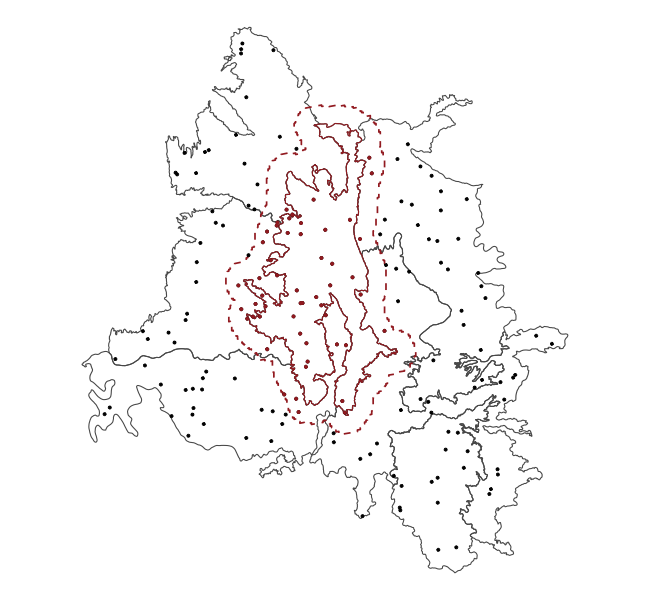
\includegraphics[width = .7\textwidth]{figures/buffer_example.png}
    \caption{Example showing how observations are selected within a region's buffer zone. Seven arbitrary regions represented as polygons contain 169 observations represented as points. During the regional modeling process, a model is built for each of the seven regions. For this example, all points within 50km of a region are used to build each model. For the highlighted region, all observations within a 50km buffer zone (dashed line) are used to build that region's model. Highlighted points are observations used to build the highlighted region's model.}
    \label{fig:buffer_example}
\end{figure}

Simply making predictions within each $\mathcal{R}_{p_i}$ using each corresponding $f_{p_i}(\pmb{X})$ results in noncontinuous predictions at region boundaries. Regional border smoothing results in continuous predictions for the entire space by taking a weighted average of the predictions provided by each $f_{p_i}(\pmb{X})$. The smoothed global prediction surface is continuous, but not necessarily differentiable.

\subsection{Smoothing at borders}

Let $\hat{y}_{1}, \hat{y}_{2}, ..., \hat{y}_{m}$ represent predictions from regional models $f_{p_1}(\pmb{x}^*), f_{p_2}(\pmb{x}^*), ..., f_{p_m}(\pmb{x}^*)$ for location of interest $\pmb{x}^*$ where $\pmb{x}^*$ represents both spatial and non-spatial information. A final prediction $\hat{y}'$ is calculated by the weighted average of each $\hat{y}$, i.e.,

\begin{equation}
    \hat{y}' = \frac{\sum_{i=1}^m w(d_i|S)\hat{y}_{i}}{\sum_{i=1}^m w(d_i|S)}.
    \label{eq:smooth}
\end{equation}

The weights are calculated based on the smallest great-circle distances ($d_{1}, d_{2}, ..., d_{m}$) between the location of $\pmb{x}^*$ and the boundaries of $\mathcal{R}_{p_1}, \mathcal{R}_{p_2}, ..., \mathcal{R}_{p_m}$. If $\pmb{x}^*$ is located within a region, the distance between $\pmb{x}^*$ and that region is $0$. The weight $w(d_i|S)$ given to $\hat{y}_{i}$ is non-zero when $d_{i}$ is within some threshold $S$, i.e.,

\begin{equation}
    w(d_i | S) = 
    \begin{cases} 
        \left( \frac{S - d_{i}}{S} \right)^2 & d_{i} \leq S\\ 
        0 & d_{i} > S.
    \end{cases}
    \label{eq:weight}
\end{equation}

Consider now the special case when a prediction is made in region $j$ and $d_{i\ne j} > S$, then $w(d_{i \ne j}|S) = 0$ and Equation \ref{eq:smooth} reduces to $\hat{y}' = \hat{y}_{j}$. As prediction location in region $j$ approach $\mathcal{R}_{p_k}$, then the weight of $\hat{y}_{k}$ increases gradually and $\hat{y}' = \frac{ \hat{y}_{j} + \left(\left(S - d_{k}\right)/S\right)^2 \hat{y}_{k}}{1 + \left(\left(S - d_{k}\right)/s\right)^2}$. At the border of regions $j$ and $k$, $\hat{y} = \left(\hat{y}_{j} + \hat{y}_{k}\right) / 2$. Finally, as prediction locations progress into $\mathcal{R}_{p_k}$, weights for $y_{i_j}$ decrease gradually to zero and $\hat{y}' = \frac{\left(\left(S - d_{j}\right)/S\right)^2 \hat{y}_{j} + \hat{y}_{k}}{\left(\left(S - d_{j}\right)/S\right)^2 + 1}$. All locations within $S$ of a region are referred to as the smoothing zone for that region.

\subsection{Standard error approximations}

The smoothing approach described in this paper represents a spatially weighted ensemble of model predictions along region boundaries, with each model (possibly) estimating prediction standard error (SE) or variance. There is no consensus in the literature on how SE should be calculated for ensemble model predictions. The methods for SE calculation that do exist tend to be specific to model type (e.g. \cite{wager2014confidence}) or averaging approach (e.g. \cite{hoeting1999bayesian}). For this reason, the method for estimating SE in \pkg{remap} relies on the general properties of variance for the summation of random variables.

Suppose that each $\hat{y}_i$ is an unbiased estimate from of $f_{p_i}(\pmb{x}^*)$ with the SE of $\hat{y}_i$ represented as $\hat{\sigma}_i$. Then the combined model SE for $\hat{y}'$ can be represented as 
%
\begin{equation}
     \hat{\sigma}' = \sqrt{\frac{\sum_{i=1}^m w(d_i|S)^2\hat{\sigma}_{i}^2 + \sum_{i=1}^m\sum_{j<i} 2w(d_i|S)w(d_j|S)\rho_{ij}\hat{\sigma}_{i}\hat{\sigma}_{j}}{\left(\sum_i w(d_i|S)\right)^2}},
\end{equation}
%
where $\rho_{ij}$ represents the correlation between predictions for model $i$ and $j$. One primary difficulty with estimating $\hat{\sigma}'$ in the smoothing zones is a lack of information regarding $\rho_{ij}$. It is highly likely that SE estimates are correlated for models in adjacent regions. In the absence of a computationally efficient and theoretically robust estimate for $\rho_{ij}$ the Cauchy–Schwarz inequality can be used to provide an upper bound on $\hat{\sigma}'$ given as 
%
\begin{equation}
     \hat{\sigma}' \le \sqrt{\frac{\sum_{i=1}^m w(d_i|S)^2\hat{\sigma}_{i}^2 + \sum_{i=1}^m\sum_{j<i} 2w(d_i|S)w(d_j|S)\hat{\sigma}_{i}\hat{\sigma}_{j}}{\left(\sum_i w(d_i|S)\right)^2}},
     \label{eq:cs_in}
\end{equation}
%
where $\rho_{ij}$ has been replaced with a constant value of one. 

The \pkg{remap} package provides a method for estimating the upper bound of the prediction SE using the inequality specified in (\ref{eq:cs_in}). It is important to note that it may not always be appropriate to combine model SE  estimates in this way. This is particularly true for models that ignore spatial autocorrelation. It is also important to remember that the primary focus of \pkg{remap} is to provide a practical approach for smoothing model predictions, and not to preserve the theoretical integrity of the SE estimates. It is up to the end user to determine that the SE calculations are valid and appropriate for their modeling purposes.  

\subsection{A note on smoothing}

The ``smoothing'' described throughout this article refers to smoothing in the colloquial sense. A continuous prediction surface is created with a steady transition between regions. The prediction surface is not always differentiable. If a region is not convex, the rate of change in the distance to a region can shift suddenly at locations that are equidistant to different parts of the region. Figure \ref{fig:nondiff} shows an example of a prediction surface near a non-convex region where the prediction surface is not differentiably smooth.

\begin{figure}[htbp]
    \centering
    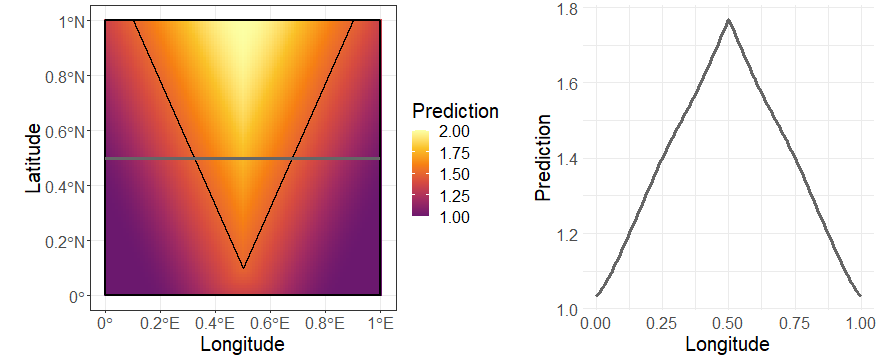
\includegraphics[width = \textwidth]{figures/nondiff.png}
    \caption{Example of where predictions are not differentiable near non-convex regions. The bottom region predicts a constant value of one and the top region predicts a constant value of two with a smoothing zone of 40 km ($\approx 0.36$\textdegree). The gray line shows predicted values along the 0.5\textdegree N transect. This example illustrates that the smoothing approach always produces continuous predictions, but differentiability is dependent on the shape of the polygon partition. }
    \label{fig:nondiff}
\end{figure}

Since each region is a closed set of points, $d_i$ is continuous. It therefore follows that the weight function $w(d_i|S)$ described in  Equation \ref{eq:weight} is continuous as $\lim_{x\to0^{+}} w(x|S) = w(0|S) = 1$ and $\lim_{x\to S^{-}} w(x|S) = w(S|S) = 0$ for $x \in [0, \infty)$ and $S > 0$. Since the right side of Equation \ref{eq:smooth} is the multiplication and addition of continuous functions, it is guaranteed to have $\max\left(w(d_i|S)\right) > 0$ as long as $\pmb{x}^*_s$ is within $S$ units of any $\mathcal{R}_p$ and it follows that Equation $\hat{y}'$ is also continuous. Given continuous predictions as a function of location for each region, the regional border smoothing method is guaranteed to be continuous for any location within the smoothing zone of at least one region. Once all $d_i > S$, then the denominator of $y'$ is equal to zero, which means $y'$ is no longer well-defined. As long as all of the data $\pmb{X}$ are located within $\mathcal{R}_p$, any prediction location outside of $\mathcal{R}_p$ is spatial extrapolation that is generally discouraged.


\section{remap}

The R package \pkg{remap} is an implementation of the regional border smoothing approach to spatial modeling. The function \code{remap} creates a set of regionalized models given:
\begin{itemize}
    \item A set of observations as spatially projected or geographic points.
    \item A set of regions as spatially projected or geographic polygons.
    \item A desired buffer zone distance.
    \item A modeling function to apply to observations in each region.
\end{itemize} Predictions can be made on new observations given a regionalized model and the smoothing parameter \code{smooth} used for weighted averages in smoothing zones (variable $S$ in Equation \ref{eq:weight}). Detailed descriptions of function parameters can be found in the package documentation. Some working examples using the \pkg{remap} package are provided via the vignette which accompanies the package. The development version of the code for \pkg{remap} can be found at \url{https://github.com/jadonwagstaff/remap}.

\subsection{Calculating distances}

The weights for regional predictions require the distances from all observations to the boundary of each region. The modeling process of the \code{remap} function also requires the distances from all observations to each region to assign the correct observations to each regional model. The process of fine-tuning a model can result in recalculating these distances many times. To avoid recalculating distances, the function \code{redist} is included in the \pkg{remap} package to pre-compute the distances from a given set of observations to a given set of regions. These pre-computed distances can be supplied as a parameter to the \code{remap} function to reduce computational time while fine-tuning models.

Calculating distances in the \pkg{remap} package takes advantage of tools already available for spatial analysis in the R package \pkg{sf} \citep{pebesma2018}. The function \code{sf::st\_distance} is used to find either Euclidean or great-circle distances depending on the spatial projection of the locations and regions. The \code{sf::st\_distance} function uses the \pkg{S2} geometry library \citep{google2020} when calculating great-circle distances. The \pkg{S2} geometry library is designed specifically to efficiently compute distances between nearby objects given large sets of geographic data. Regardless, calculating distances can still take a lot of computational time if the regions are complex and/or there are a lot of observations.

The na\"ive approach to regional border smoothing is to find all distances between each location and each region. This approach may be necessary during the modeling process if any region does not contain a required minimum number of observations (detailed in the implementation considerations section). If predictions are being made using new observations, then distances do not need to be calculated between every observation and every region.

Because the weight for predictions in different regions is zero when the distance to those regions is greater than the smoothing parameter (Equation \ref{eq:weight}), distances do not need to be calculated between \emph{every} region and \emph{every} prediction location. To determine which observations require distance calculations, an approximate polygon is constructed that encompasses the original region plus the smoothing zone around the region. The function \code{sf::st\_within} is used to determine which observations are within the new polygon and equivalently, which observations are within the smoothing zone of the original region. Observations in the approximate polygon become candidates for precise distance calculations. 


An approximate polygon that contains a region and the region's smoothing zone is created using the \code{sf::st\_buffer} function. For geographic coordinates, \code{sf::st\_buffer} requires a buffer value in degrees. Since the great-circle distance between a unit degree of longitude changes with latitude, Equation \ref{eq:km_per_degree} is used to find $c$: the shortest distance (measured in kilometers) required to move one degree longitude at the observation in the data set that is nearest to a geographical pole. The set $\pmb{\lambda}$ is the set of Latitude values of the observations and 6380 km is the radius of the earth at a pole  (rounded down). A sufficient buffer value in degrees for \code{sf::st\_buffer} is calculated by dividing the smoothing zone length in km by $c$. The resulting buffered polygon contains all of the observations within the smoothing zone of the original polygon,

\begin{equation}
    c = \frac{\pi * 6350}{180} * cos\left(\frac{\pi * \max\left(|\pmb{\lambda}|\right)}{180}\right).
    \label{eq:km_per_degree}
\end{equation}

Assuming each region contains a sufficient number of observations to fit each regional model, the same process used for reducing the number of distance calculations for model predictions can be used to reduce the number of distance calculations required for model training. The function \code{redist} is able to restrict distance calculations to only observations within a certain buffer zone or smoothing zone of each region using the \code{max\_dist} parameter. This eliminates the need to calculate distances to points with a known weight of zero when smoothing.



\subsection{Practical implementation considerations}

Reliable regression results depend upon sufficient sample sizes, which differ based on the variability of the response and dimensionality of the inputs. A strict (and obvious) minimum sample size for the \pkg{remap} function is one observation per region, though this threshold will rarely, if ever, ensure reasonable results. An additional parameter \code{min\_n} is included in the \code{remap} function to specify a minimum number of observations be used to build each model. If a region and the buffer around that region do not contain the minimum number of observations specified, the \code{min\_n} observations closest to the boundaries of the region are used to train that region's model.

The \pkg{remap} package has the ability to make predictions outside of all modeling regions. If the prediction location is within the smoothing zone of a region, then Equation \ref{eq:smooth} applies and the nearest region will have the most weight. If the prediction location is outside the smoothing zone of all regions, then the model from the closest region is used to make a prediction. This may result in non-continuous transitions in predictions when the closest region changes across geographic space, but this is only possible at locations outside of the smoothing zone of all regions. As a general rule, extrapolation of predictions to a location beyond those represented in the input data is not recommended. See Figure \ref{fig:gap} for a visual depiction of how predictions behave outside of all modeling regions.

\begin{figure}[htbp]
    \centering
    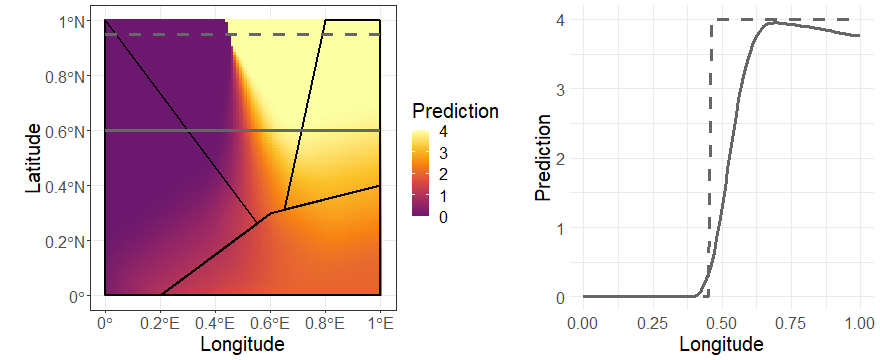
\includegraphics[width = \textwidth]{figures/gap.png}
    \caption{Example of what happens when predictions are made outside of any modeling region. The gray line shows predicted values along the 0.6\textdegree N transect. The dashed gray line shows predicted values along the 0.95\textdegree N transect. The left region predicts a constant 0, the bottom region predicts a constant 2, and the right region predicts a constant 4. Smoothing zone is 35 km ($\approx 0.32$\textdegree).}
    \label{fig:gap}
\end{figure}

The ability to predict outside of all regions means that the \pkg{remap} package can make smooth predictions across small gaps at polygon borders, provided the gaps are no larger than two times the smoothing zone distance. This encourages the use of \code{rgeos::gSimplify} \citep{rgeos2020} or \code{sf::st\_simplify} \citep{pebesma2018} to simplify complex polygons and ease the computational burden associated with distance calculations, even if those simplifications slightly compromise the topology of the original geometry. 


\section{Applications}
\subsection{Design snow loads}

Snow loads are obtained from weather stations throughout the United States in the National Oceanic and Atmospheric Administration’s (NOAA) Global Historical Climatology Network \citep{menne2012}. Snow loads are either measured directly, or estimated from measured snow depth using a depth to load conversion model. Engineers have historically used estimates of 50-year ground snow loads when designing structures. The 50-year snow load is traditionally obtained by fitting a probability distribution to yearly maximum snow load measurements and extracting the 98\textsuperscript{th} percentile. A recent effort by the American Society of Civil Engineers has resulted in a new set of 50-year ground snow loads at 7964 measurement locations \citep{bean2021-report}. 

\subsection{Building a geospatial snow load model with remap}

Building design requirements call for continuous maps that estimate design loads between measurement locations. This has historically been accomplished using various mapping techniques \citep{Tobiasson2002, Liel2017, Bean2019}. The problem is that the relationship between predictor variables and snow load can change drastically on a continental scale. For example, the typical loads at 1500 meter elevation in the Rocky Mountains of Montana are much lower than loads at 1500 meters in the Cascade Mountains of Washington State (Figure \ref{fig:elevation}). Commonly used geospatial models for mapping are not well suited for the nonstationary nature of this problem.

\begin{figure}[htbp]
    \centering
    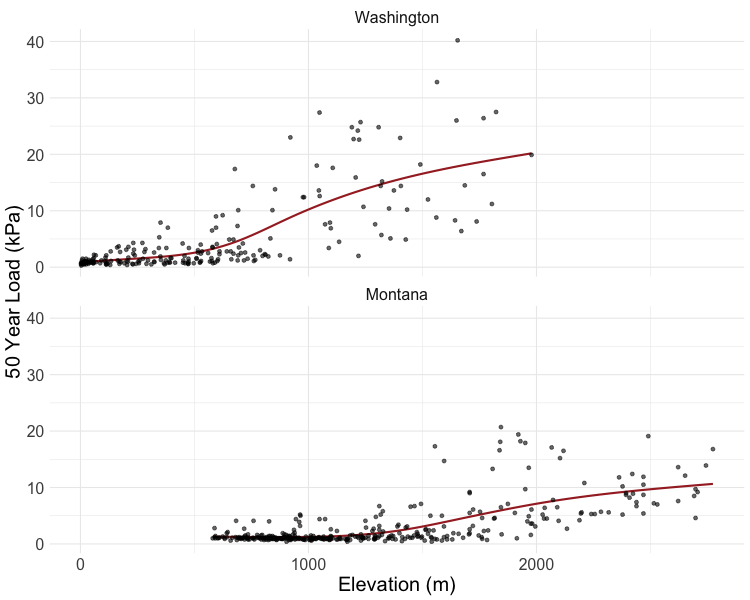
\includegraphics[width = .8\textwidth]{figures/elevation_plot.png}
    \caption{50-year events for measurement locations within Washington and Montana. Trend lines are fit with cubic regression splines. In both regions, loads eventually increase  as elevation increases, but the inflection points are about 1000 m apart and the rate of change is different. This demonstrates the need for an approach which adapts to the changing relationship between predictor variables and response in different regions.}
    \label{fig:elevation}
\end{figure}

Snow loads are typically assumed to share a log-linear relationship with elevation. This relationship can be modeled directly using ordinary least squares (OLS), which ignores any potential spatial dependencies among the observations. A generalized additive model (GAM) built with the \pkg{mgcv} R package \citep{wood2011} characterizes the log of 50-year loads as a function of elevation and a spatial smoother called splines on the sphere \citep{Wood2003}. Universal kriging interpolates values using a Gaussian process model after accounting for the log-linear trend in elevation. Variograms are individually fit within each region using the \pkg{automap} R package \citep{hiemstra2009}.

Geographic regions defined by the US Environmental Protection Agency (EPA) define regions with similar ecology and climate called eco-regions \citep{cec1997}. The eco-regions provide a natural partition of the conterminous United States and give no regard to political boundaries. Snow load can be modeled using observations within each eco-region where the relationship between predictor variables and the response are more consistent on a local level. The \pkg{remap} package facilitates modeling in separate eco-regions and creates a smooth model on the national scale. There are 86 eco-regions that fall within the conterminous United States, so 86 separate models are built using the \code{remap} function with a buffer zone of 50 km and a \code{min\_n} of 150 observations. The regional models are smoothed to a single continuous model using a \code{smooth} parameter of 25 km.

The following code demonstrates how \code{remap} is used to build these models. The script and data for the following examples are provided as supplementary materials with this article. The example data include three \code{"sf"} objects: a spatial points data frame with 50-year snow loads at locations within the US and Canada (\code{loads}), a spatial polygons data frame of eco-regions (\code{eco3}), a spatial polygon of the conterminous United States (\code{cont\_us}), and a \code{"raster"} object with elevations comprising a 0.8 km grid over the conterminous United States (\code{grd}).

\begin{example}
library(tidyverse)
library(sf)
library(raster)
library(mgcv)
library(automap)
library(gstat)
library(remap)
load("wagstaff-bean.RData")
\end{example}

The eco-regions have more complex borders than is necessary for this problem, so they can be simplified to the same extent as shown in Figure \ref{fig:simplification}.

\begin{example}
eco3_simp <- eco3 %>%
  sf::st_simplify(dTolerance = 10000) %>%
  dplyr::filter(!sf::st_is_empty(.)) %>%
  sf::st_cast("MULTIPOLYGON")
\end{example}

% polygon figure
\begin{figure}[ht]
    \centering
    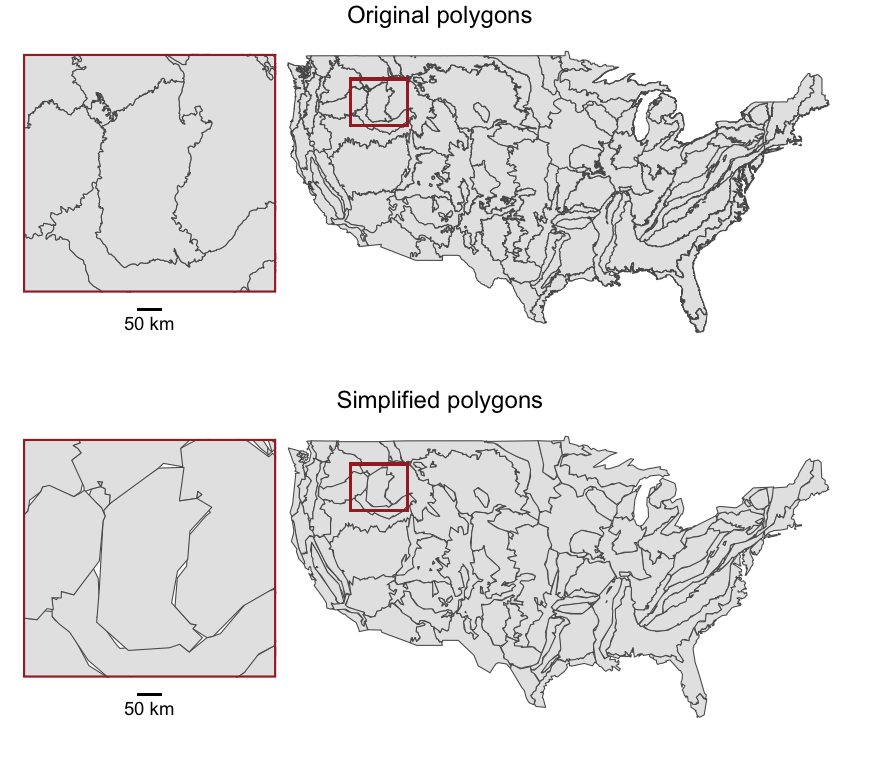
\includegraphics[width = \textwidth]{figures/polygon_simplification.png}
    \caption{Results of simplification of eco-regions. The highlighted region is an area with some of the most severe gaps between polygons. Notice that the width of the gaps are still much smaller than two times the smoothing parameter ($2 \times 25$ km).}
    \label{fig:simplification}
\end{figure}

Since multiple models are built with the same set of measurement locations, pre-calculating the distances from measurement location to region boundaries can save some computational time.

\begin{example}
eco3_dist <- redist(loads, regions = eco3_simp, region_id = ECO3)
\end{example}

Linear models and GAMs are easiest to build with remap. The \code{remap} function accepts additional arguments for a selected model function but passes the spatial data to the function as an unnamed parameter. Since the \code{data} parameter is the second parameter of the \code{stats::lm} function, we need to formally specify the first argument of the function (i.e. the \code{formula} parameter) to pass along to \code{stats::lm}, rather than relying on the \code{stats::lm} function defaults. Otherwise the data for each sub-region will be sent as the wrong parameter.

\begin{example}
lmod <- remap(loads, regions = eco3_simp, region_id = ECO3,
              buffer = 50, min_n = 150,
              distances = eco3_dist,
              model_function = stats::lm,
              formula = log(EVENT50) ~ ELEVATION)
              
lmod
#> remap model with 86 regional models
\end{example}


The \code{lmod} object has class \code{"remap"} and contains a \code{models} object and a \code{regions} object. The \code{models} object is a list of \code{gam} models where the model names correspond to each modeling region ID. The \code{regions} object is an \code{"sf"} multipolygon object with one row per region and the first column is the region IDs.

\begin{example}
head(names(lmod$models), 3)
#> [1] "10.1.2" "10.1.3" "10.1.4"

class(lmod$models[[1]])
#> [1] "lm" 

head(lmod$regions, 3)
#> Simple feature collection with 3 features and 1 field
#> Geometry type: MULTIPOLYGON
#> Dimension:     XY
#> Bounding box:  xmin: -121.3721 ymin: 40.15434 xmax: -105.4847 ymax: 49.39082
#> Geodetic CRS:  WGS 84
#>     ECO3                           geom
#> 1 10.1.2 MULTIPOLYGON (((-115.8435 4...
#> 2 10.1.3 MULTIPOLYGON (((-120.5262 4...
#> 3 10.1.4 MULTIPOLYGON (((-108.8632 4...
\end{example}


Similar to the \code{stats::lm} function, the \code{mgcv::gam} function needs a \code{formula} parameter and a \code{family} parameter passed to the \code{remap} function since \code{data} is the third parameter of \code{mgcv::gam}. In this example a wrapper function for \code{mgcv::gam} is written to allow a custom predict function which either return predicted values (\code{se.fit = FALSE}) or standard errors (\code{se.fit = TRUE}). 

\begin{example}
gam_wrap <- function(data, ...) {
  model <- mgcv::gam(data, ...)
  class(model) <- "gam_wrap"
  return(model)
}

predict.gam_wrap <- function(object, data, se.fit = FALSE) {
  class(object) <- "gam"
  if (se.fit) { # return standard errors
    return(predict(object, data, se.fit = TRUE)$se.fit)
  } else { # return predictions
    return(predict(object, data))
  }
}

gm <- remap(loads, 
            regions = eco3_simp, region_id = ECO3,
            buffer = 50, min_n = 150,
            distances = eco3_dist,
            model_function = gam_wrap,
            formula = log(EVENT50) ~ s(ELEVATION, k = 15) +
              s(LATITUDE, LONGITUDE, bs = 'sos', k = 75),
            family = stats::gaussian)

predict(gm, loads[1:3, ], smooth = 25)
#> [1] -0.003297382  0.132882034 -0.170530457

predict(gm, loads[1:3, ], smooth = 25, se = TRUE, se.fit = TRUE)
#> Upper bound for standard error calculated at each location. 
#> Reminder: make sure that the predict function outputs a vector of standard
#> error values for each regional model in your remap object.
#> [1] 0.3177003 0.3383906 0.2142151

\end{example}


The kriging example requires a bit more work to implement in \pkg{remap} since the \code{automap::autoKrige} and \code{gstat::krige} functions do not accept data as an \code{"sf"} object. A custom modeling function can be written to pass to \pkg{remap} and a custom predict function can be written for \pkg{remap} to use for predictions.

\begin{example}
projection <- sf::st_crs("+proj=laea +x_0=0 +y_0=0 +lon_0=-100 +lat_0=45")

krig <- function(data, formula) {
  data <- data %>%
    sf::st_transform(projection) %>%
    sf::as_Spatial()
  
  out <- list(data = data, formula = formula)
  class(out) <- "krig"
  
  return(out)
}

predict.krig <- function(object, data) {
  if (nrow(data) == 0) return(NULL)
    data <- data %>%
      sf::st_transform(projection) %>%
      sf::as_Spatial()
    
    variogram_object <- automap::autofitVariogram(
      formula = object$formula, 
      input_data = object$data,
      model = "Sph")
    
    k <- gstat::krige(formula = object$formula, 
                      locations = object$data,
                      newdata = data, 
                      model = variogram_object$var_model,
                      debug.level = 0)
    
    return(k$var1.pred)
}

kg <- remap(loads, 
            regions = eco3_simp, region_id = ECO3,
            buffer = 50, min_n = 150,
            distances = eco3_dist,
            model_function = krig,
            formula = log(EVENT50) ~ ELEVATION)
\end{example}

Since the buffer distance is greater than the smoothing distance, the resulting \code{"remap"} object can be used to interpolate the same way that a global kriging model interpolates between points.

\begin{example}
loads_us <- sf::st_filter(loads, cont_us)

kg_preds <- exp(predict(kg, loads_us, smooth = 25))

all(dplyr::near(kg_preds, loads_us$EVENT50))
#> [1] TRUE
\end{example}


Snow load modeling methods are compared in Table \ref{tab:standard_cv_50} using national scale models and models built with the \pkg{remap} package on  EPA Level III Eco-Regions \citep{cec1997}. Table \ref{tab:standard_cv_50} shows that the \pkg{remap} package framework improves the cross validated accuracy of every spatial modeling method. This demonstrates that the \pkg{remap} package has the ability to generally improve modeling results, as improvements are not isolated to a single spatial modeling case. Even though the regional models are made up of 86 different regional models, the estimated 50-year loads are smooth across the prediction surface.

\begin{table}[htbp]
    \centering
    \begin{tabular}{lrrr}
        \toprule
        \multirow{2}{*}{Model} & \multicolumn{2}{c}{MSE $\times10^2$} & \multirow{2}{*}{Improvement}\\
        \cline{2-3}
        & National & Regional & \\
        \midrule
        GAM & 8.1 & 5.5 & 32\%\\
        Kriging & 7.2 & 5.9 & 18\%\\
        OLS & 89.3 & 17.8 & 80\%\\
        \bottomrule
    \end{tabular}
    \caption{Ten fold cross-validation results from modeling the log of 50-year snow loads. Mean squared error (MSE) is multiplied by $10^2$ for readability. Improvement is (national - regional) / national.}
    \label{tab:standard_cv_50}
\end{table}

\subsection{Computational challenges}

National snow load maps require a sufficiently fine resolution to be feasibly used to design buildings in topographically complex areas. To accomplish this, snow load maps are created that match the resolution of PRISM climate output \citep{prism2020}, which maps at a 0.8 km resolution for the conterminous United States. This means that predicted snow loads are calculated at 12,113,556 locations using a model created by the \pkg{remap} package with 86 different regions. Elevation values for the grid are obtained from the United States Geological Survey \citep{USGS2020}.

Since the \pkg{remap} package uses the distances between prediction locations and regions to make a smooth model, calculating these distances is a potential bottleneck in the prediction process. Also, since the prediction area is so large, geographic coordinates rather than projected coordinates must be used to find distances. Prior to \pkg{sf} version 1.0.0 \citep{pebesma2018}, the \pkg{S2} geometry library \citep{google2020} had not been implemented. Without the \pkg{S2} geometry library, simply calculating all geographic distances would have taken nearly half a year to run on a typical personal computer, as illustrated in Table \ref{tab:runtime}. The test computer used for Table \ref{tab:runtime} has 16 GB of RAM and an Intel Core I7-7820HQ CPU which runs at 2.9 GHz. Maps for the national design snow loads were developed before \pkg{S2} had been integrated into \pkg{sf}, so the steps described later in this section had previously been necessary to use \pkg{remap} to build these maps.

% Run time table
\begin{table}[htbp]
    \centering
    \begin{tabular} {lrrr}
        \toprule
        \multirow{2}{*}{Remedial steps} & \multicolumn{3}{c}{Run time in hours}\\
        \cline{2-4}
        & Geographic \hspace{.1em} & Geographic (\pkg{S2}) \hspace{.1em} & Projected \hspace{.1em} \\
        \midrule
        None &  4200$^*$ & 8.1$^*$ & 100.0$^*$\\
        Simplify polygons & 14$^*$ & 2.3$^*$ & 1.0 \hspace{.1em} \\
        \hspace{0.2em} + set \code{max\_dist} to 25 km  & 1.1 \hspace{.1em} & 0.3 \hspace{.1em} & 0.8 \hspace{.1em} \\
        \hspace{0.2em} + run in parallel on 4 cores & 0.8 \hspace{.1em} & 0.3 \hspace{.1em} & 0.8 \hspace{.1em} \\
        \bottomrule
    \end{tabular}
    \caption{Run times for \code{redist} to calculate geographic and projected distances from 0.8 km grid points to 86 different eco-regions (polygons) in the conterminous US. Remedial steps are additive, i.e., each row in the table includes all previous remedial steps. $^*$ Approximate run time based on random sample of 10,000 grid points.}
    \label{tab:runtime}
\end{table}

The first step to reduce the run time for distance calculations is to simplify the polygons as discussed in the implementation considerations. Using a tolerance of 10000 with the function \code{sf::st\_simplify}, the size of the polygons are reduced from 21 MB to 0.2 MB. The results of polygon simplification are visualized in Figure \ref{fig:simplification}. When making predictions, the \code{smooth} parameter is set to 25 km; therefore, the \code{max\_dist} parameter of \code{redist} can be set to 25 km to further reduce run time. The distances may also be calculated in parallel; however, on the test computer the improvements are marginal. The relevant distances may be calculated for all points using great circle distance in as fast as 20 minutes (Table \ref{tab:runtime}). This tremendous computational speed-up is made possible by the ability of the \pkg{remap} package to smoothly fill in the gaps that occur in aggressively simplified polygons. 

Here is an example of the code used to find distances from grid points to eco-regions. Due to space and time constraints, the 0.8 km prediction grid is aggregated to a 7.2 km grid (\code{grd}) over the conterminous United States. The grid is also converted to an \code{"sf"} spatial points data frame for use with \pkg{remap}.

\begin{example}
ag_grd <- grd %>%
  raster::aggregate(9) %>%
  raster::rasterToPoints() %>%
  as.data.frame() %>%
  mutate(LONGITUDE = x, LATITUDE = y) %>%
  sf::st_as_sf(coords = c("x", "y"), crs = 4326) %>%
  filter(sf::st_intersects(., cont_us, sparse = FALSE)[,1])

grd_dist <- redist(ag_grd, regions = eco3_simp, region_id = ECO3, max_dist = 25)
\end{example}

Smoothed regional predictions are made automatically by using the generic \code{predict} function on a \code{"remap"} object and setting the \code{smooth} parameter to value greater than zero. Below is an example of predicting values on the grid points using the 50-year load regionalized GAM model. Since we already calculated distances from \code{grd} to \code{eco3\_simp}, the \code{grd\_dist} object can be passed to the \code{distances} parameter of the \code{predict} function. The distance matrix is optional and \code{remap} will calculate distances internally if not provided with a distance matrix. Predictions are smoothed to 25 km on either side of each border. Note that predictions from \code{gm} are on the log scale.

\begin{example}
gm_preds <- predict(gm, ag_grd, smooth = 25, distances = grd_dist)
gm_preds <- exp(gm_preds)
\end{example}

Here, the predictions from the regionalized GAM reveal some extrapolation issues when making predictions at elevations outside of the range of available data within each sub-region. To get a better visualization of the predictions, the predicted values can be truncated to the range observed in the input data. 

\begin{example}
range(gm_preds)
#> [1]   0.04273189 444.34484622
range(loads$EVENT50)
#> [1]  0.1 40.2

gm_preds[gm_preds > 40.2] <- 40.2
gm_preds[gm_preds < 0.1] <- 0.1
\end{example}

The smooth predictions from the \code{gm} model are visualized in Figure \ref{fig:snowload_map} with the following code.

\begin{example}
ggplot(cont_us) +
  geom_tile(data = ag_grd %>% dplyr::mutate(EVENT50 = gm_preds), 
            aes(x = LONGITUDE, y = LATITUDE, fill = EVENT50)) +
  geom_sf(fill = NA, color = NA) +
  scale_fill_viridis_c(option = "inferno",
                       trans = "log10",
                       breaks = c(0.1, 1, 7, 40),
                       labels = c("0.1 kPa", "1 kPa", "7 kPa", "40 kPa"),
                       name = "50-year event") +
  theme_void()
\end{example}

% load map
\begin{widefigure}[htbp]
    \centering
    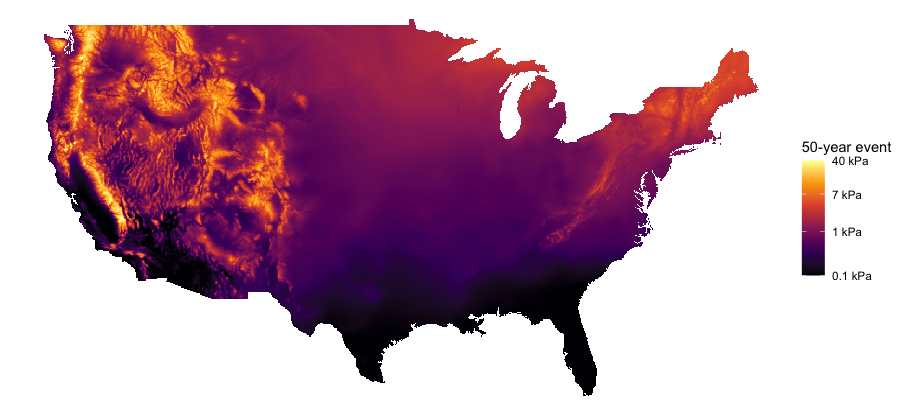
\includegraphics[width = \textwidth]{figures/snowload_map.png}
    \caption{Prediction map for 50-year loads from the regional GAM model built with the \pkg{remap} package using 7,936 observations wthin 86 eco-regions. GAM models are built using a buffer zone of 50 m and predictions are smoothed using a smoothing zone of 25 m. Values are restricted to be within the range of values observed in the load data. This figure illustrates how \pkg{remap} functions can be used to create continuous predictions of snow loads for all of the Conterminous United States.}
    \label{fig:snowload_map}
\end{widefigure}

\subsection{Utah snowpack}

The state of Utah assesses snow water content or snowpack every April 1\textsuperscript{st} to plan for yearly water resource availability. These measurements are much more variable than the 50-year snow loads since the values are based on a single measurement at each location instead of the 98\textsuperscript{th} percentile of a distribution fit to annual maximum values at each location. This example uses direct measurements of the water content made via Snowpack Telemetry (SNOTEL) stations included in NOAA's Global Historical Climatology Network \citep{menne2012}. In addition to SNOTEL station data, Snow Course data collected by the National Water and Climate Center are also included in the data set \citep{NRCS2017}. SNOTEL and Snow Course data measure the water equivalent of snow depth (WESD) and are located in the mountainous areas of Utah above 1777 m elevation. This negates the need to estimate water content from snow depth, which is typically the case when measuring snow at non-mountainous locations in the state.

SNOTEL stations and Snow Course data within 100 km of the border of Utah are included in the data set. There are 3511 April 1\textsuperscript{st} WESD observations available for modeling which range from 0 to 1746 mm of water. The observations have 178 unique locations and span 30 years (1986-2015). Each year is modeled separately with no regard for any temporal correlations and each year has at least 97 observations.

Models for GAM, kriging, and OLS are created using the same model structure as the national snow load example, but a different response variable. Since there are 142 zero values for WESD within the data, the log of (WESD + 1) is used as the response variable for the April 1\textsuperscript{st} snowpack. Predictions are also constrained to be between [1, max(WESD)] to avoid excessive extrapolation. The regions used for regional modeling are watershed boundaries defined by the USGS \citep{USGS2020_2}. Watersheds are defined by a hierarchy of hydrologic unit codes (HUC) with a two-digit designation for continental scale watersheds (HUC2) and a four-digit designation that partitions each HUC2 region (HUC4). There are four HUC2 regions and 12 HUC4 regions within the boundaries of the state of Utah (see Figure \ref{fig:utah_regions}). A buffer zone of 20 km, a smoothing parameter of 10 km, and a \code{min\_n} of 30 observations are used when modeling over both HUC2 and HUC4 regions with the \code{remap} function.

% utah figure
\begin{figure}[htbp]
    \centering
    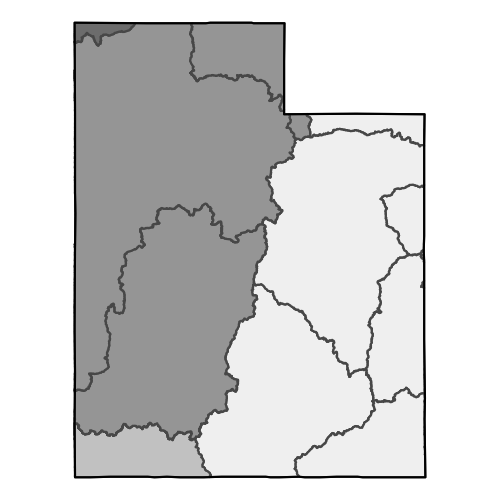
\includegraphics[width=.46\textwidth]{figures/utah_regions.png}
    \caption{HUC4 regions (lines) and HUC2 regions (shades) in Utah.}
    \label{fig:utah_regions}
\end{figure}


The following code shows how \pkg{remap} models are built for the 2011 snowpack values using HUC2 watershed regions. Included in the supplied example data are an \code{sf} points data frame with snowpack Utah snowpack values (\code{utapr1}, and an \code{sf} polygons data frame of HUC2 and HUC4 watersheds within Utah (\code{utws}). Note that the maximum number of knots (\code{k}) in the GAM formula are reduced to accommodate a smaller \code{min\_n} in the \code{remap} function.

\begin{example}
utsp2011 <- utapr1 %>%
  dplyr::filter(YEAR == 2011) %>%
  dplyr::mutate(WESD = WESD + 1)

utlmod <- remap(utsp2011, 
                regions = utws, region_id = HUC2,
                buffer = 20, min_n = 30,
                model_function = stats::lm,
                formula = log(WESD) ~ ELEVATION)
                
utgm <- remap(utsp2011, 
              regions = utws, region_id = HUC2,
              buffer = 20, min_n = 30,
              model_function = mgcv::gam,
              formula = log(WESD) ~ s(ELEVATION, k = 5) +
                s(LATITUDE, LONGITUDE, bs = 'sos', k = 20),
              family = gaussian)
              
utkg <- remap(utsp2011, 
              regions = utws, region_id = HUC2,
              buffer = 20, min_n = 30,
              model_function = krig,
              formula = log(WESD) ~ ELEVATION)
\end{example}

Table \ref{tab:standard_cv_apr1} shows that the gains in accuracy are more modest in this application than in the national example shown previously. This is expected as the partitions are on the state level instead of the national level. Nevertheless, the consistent improvement in accuracy at various scales using different polygons and different input data highlight the general ability of the \pkg{remap} package to improve predictive accuracy without sacrificing continuity. 

\begin{table}[htbp]
    \centering
    \begin{tabular}{lrr@{}rr@{}r}
        \toprule
        \multirow{2}{*}{Model} & \multicolumn{5}{c}{MSE $\times10^2$}\\
        \cline{2-6}
        & State & \multicolumn{2}{c}{HUC2} & \multicolumn{2}{c}{HUC4}\\
        \midrule
        GAM & 88 & 75 & (15\%) & 78 & (11\%) \\
        Kriging & 90 & 87 & (3\%) & 83 & (8\%) \\
        OLS & 140 & 111 & (21\%) & 89 & (36\%)\\
        \bottomrule
    \end{tabular}
    \caption{Ten fold cross-validation mean squared error from modeling log(WESD + 1) for Utah snowpack. Mean squared error (MSE) is multiplied by $10^2$ for readability. Improvement in parentheses is calculated with (state - HUC) / state.}
    \label{tab:standard_cv_apr1}
\end{table}



\section{Conclusions}

Partitioning a space for geospatial modeling is a practical approach for handling nonstationary data; however, smooth transitions in mapped values are a desirable constraint of many projects, such as the design snow load requirements set forth by the American Society of Engineers. The \pkg{remap} R package provides a ready-to-use framework for regional models with smooth transitions at region borders that overcomes the computational difficulties of na\"ive implementations.

The \pkg{remap} package creates continuous prediction surfaces by weighting regional predictions based on the proximity to region borders. Smoothing at region borders makes the package particularly equipped to handle irregularly shaped regions not well represented by their geographic centers. Because the \pkg{remap} package has the ability to smooth over small gaps formed when simplifying polygons, computation times can be drastically reduced without sacrificing the continuity of the predictions. Methods that automatically subset the number of required distance calculations further reduce computational times. This article has demonstrated accuracy improvements using the \pkg{remap} package on two separate data sets with two sets of polygon inputs. These examples highlight the feasibility of applying the \pkg{remap} framework to large spatial regression modeling problems.\\ 


\section{Acknowledgements} 

The development of \pkg{remap} was funded in part by the American Society of Civil Engineers (ASCE) and the Structural Engineering Institute in partnership with several organizations including (in alphabetical order): Factory Mutual, Metal Building Manufacturer’s Association, National Council of Structural Engineering Associations, Nucor, Simpson Gumpertz and Heger, the State of Montana, the Steel Deck Institute, the Steel Joist Institute, Structural Engineers Association of Montana, Wiss Janney and Elstner Associates. Further, the authors would like to thank Dr. Kevin Moon of Utah State University for his insight on the ensemble SE estimation problem. 


\bibliography{wagstaff-bean}

\address{Jadon Wagstaff\\
  Huntsman Cancer Institute, University of Utah\\
  Department of Oncological Sciences\\
  2000 Circle of Hope\\
  Salt Lake City, UT 84112, USA\\
  \email{jadonw@gmail.com}}

\address{Brennan Bean\\
  Utah State University\\
  Department of Mathematics and Statistics\\
  3900 Old Main Hill\\
  Logan, UT 84322, USA\\
  \email{Brennan.Bean@usu.edu}}
